% Cảm ơn Bùi Vân Anh
% Rewrite by ledangquangdangquang 30 - 9 - 2024
% Ctrl + Alt + J: SyncTeX from edit view
% Ctrl + Click: SyncTeX from read view
\documentclass{article}
\usepackage[utf8]{inputenc}
\usepackage[T5]{fontenc}
\usepackage{mathptmx} % Time New Roman
\usepackage[fontsize=13pt]{scrextend}
\usepackage[paperheight=29.7cm, paperwidth=21cm, right=2.5cm, left=3.5cm, top=2cm, bottom=2cm]{geometry}
% show line margin
% \usepackage[paperheight=29.7cm, paperwidth=21cm, right=2.5cm, left=3.5cm, top=2cm, bottom=2cm, showframe,margin=1in]{geometry}
\usepackage{graphicx}
\usepackage{float}
\usepackage{tikz}
\usetikzlibrary{calc}
\renewcommand{\baselinestretch}{1.2} % Giãn dòng 1.2
\usepackage{indentfirst} % thư viện thụt dòng 
\setlength{\parskip}{6pt} % Spacing after
\setlength{\parindent}{1cm} % Set thụt đầu dòng
\usepackage{helvet}   % Font không chân (sans-serif)
\usepackage{titlesec} % Thư viện để set up các kiểu chữ
\usepackage{stackengine} % Gói để sử dụng gạch trên chữ
\usepackage{tabularx} % Gói để căn vị trí cho bảng
\usepackage{caption} % Gói để xóa dấu hai chấm
\usepackage{amsmath} % Gói hỗ trợ xóa dấu ngoặc mặc định của phương trình (gói cho toán học)
\usepackage{lipsum} % Gói tạo chữ linh tinh
\usepackage[unicode]{hyperref} % Để bấm mục lục
\usepackage{enumitem} % Để customize đề mục tự đếm
% \usepackage{svg}
% XỬ LÝ MỤC LỤC
\renewcommand{\contentsname}{\centering MỤC LỤC} % Đổi tiêu đề và căn giữa
% XỬ LÝ ĐỀ MỤC
\setcounter{secnumdepth}{4} % Khai báo là có 4 heading
\titlespacing*{\section}{0pt}{0pt}{30pt} % Heading 1
\titleformat*{\section}{\fontsize{16pt}{0pt}\selectfont \bfseries}
\titlespacing*{\subsection}{0pt}{10pt}{0pt} % Heading 2
\titleformat*{\subsection}{\fontsize{14pt}{0pt}\selectfont \bfseries}
\titlespacing*{\subsubsection}{0pt}{10pt}{0pt} % Heading 3
\titleformat*{\subsubsection}{\fontsize{13pt}{0pt}\selectfont \bfseries \itshape}
\titlespacing*{\paragraph}{0pt}{10pt}{0pt} % Heading 4
\titleformat*{\paragraph}{\fontsize{13pt}{0pt}\selectfont \itshape}
% XỶ LÝ HÌNH VẼ 
\renewcommand{\listfigurename}{\centering DANH MỤC HÌNH VẼ} % Đổi tiêu đề và căn giữa
\renewcommand{\figurename}{\textit{\fontsize{12pt}{0}\selectfont Hình}} % Đổi tiêu đề và căn giữa
\renewcommand{\thefigure}{\textit{\fontsize{12pt}{0}\selectfont \thesection.\arabic{figure}}} 
\captionsetup[figure]{labelsep = space}
% XỬ LÝ BẢNG BIỂU
\renewcommand{\listtablename}{\centering DANH MỤC BẢNG BIỂU} % Đổi tiêu đề và căn giữa
\renewcommand{\tablename}{\textit{\fontsize{12pt}{0}\selectfont Bảng}} % Đổi tiêu đề và căn giữa
\renewcommand{\thetable}{\textit{\fontsize{12pt}{0}\selectfont \thesection.\arabic{table}}} 
\captionsetup[table]{labelsep = space}
\newcolumntype{s}{>{\centering\arraybackslash\hsize=.7\hsize}X}
\newcolumntype{a}{>{\centering\arraybackslash\hsize=1.3\hsize}X}
% XỬ LÝ PHƯƠNG TRÌNH
\makeatletter
\renewcommand{\theequation}{\textit{\fontsize{12pt}{0}\selectfont PT \thesection.\arabic{equation}}} % thay đổi đánh số phương trình mặc định 
\def\tagform@#1{\maketag@@@{\textnormal{#1}}} % Xóa dấu ngoặc quanh số phương trình
\makeatother
% XỬ LÝ ĐỊNH NGHĨA, ĐỊNH LÝ, BỔ ĐỀ
\newtheorem{theorem}{Định lý}[section]
\newtheorem{defn}[theorem]{Định nghĩa}
\newtheorem{corollary}[theorem]{Hệ quả}
\newtheorem{lemma}[theorem]{Bổ đề}
% XỬ LÝ TÀI LIỆU THAM KHẢO
\renewcommand{\refname}{\centering TÀI LIỆU THAM KHẢO}

\begin{document}
    % INPUT NỘI DUNG 
    \thispagestyle{empty} % Bỏ dấu trang

% Bìa 1 
\begin{center}
    % Tên trường     
    \textbf{\fontsize{15pt}{0pt}\selectfont TRƯỜNG ĐẠI HỌC BÁCH KHOA HÀ NỘI\\}

    % Vẽ đường thẳng 
    \vspace{-1.5ex}
    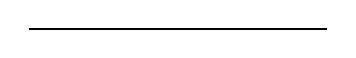
\begin{tikzpicture}
        \draw[thick] (0, 5cm) -- (3.79cm,5cm);
    \end{tikzpicture}
    
    % Chèn hình ảnh 
    \vspace{1em}
    \begin{figure}[H]
        \centering
        
\includegraphics[width=2.43cm, height=3.94cm]{image/Logo_Hust.png}
    \end{figure}
    
    % Tên Đồ án
    \vspace{1.5cm}
    {\sffamily \fontsize{21pt}{0pt}\selectfont {\textbf{ĐỒ ÁN TỐT NGHIỆP}}\\}
    \vspace{2em}
    {\sffamily \fontsize{17pt}{0pt}\selectfont {\textbf{THIẾT KẾ HỆ THỐNG TỰ ĐỘNG ĐIỀU CHỈNH NHIỆT ĐỘ TRONG THIẾT BỊ SẤY HOA QUẢ}}\\}
    % Tên 
    \vspace{2em}
    \textbf{\fontsize{11pt}{0pt}\selectfont LÊ ĐĂNG QUANG\\}
    \vspace{1ex}
    \fontsize{14pt}{0pt}\selectfont quang.ld224113@sis.hust.edu.vn\\

    \vspace{1em}
    \textbf{\fontsize{14pt}{0pt}\selectfont Ngành KT Điện tử \& Viễn thông\\}
    \vspace{1ex}
    \textbf{\fontsize{14pt}{0pt}\selectfont Chuyên ngành Điều khiển tự động \\}

    % Bảng thông tin
    \vspace{5em}
    \begin{tabular}{  l  l  r }
        \textbf{Giảng viên hướng dẫn:}&PGS. TS. Phạm Văn ABC& \fontsize{10pt}{0pt}\selectfont \stackon{Chữ ký của GVHD}{\rule{4cm}{0.4pt}} \\ [3em] 
        \textbf{Bộ môn:}&Điều khiển tự động& \\ [1ex] 
        \textbf{Trường:}&Điện - Điện tử& \\
    \end{tabular}

    % Thời gian
    \vfill

    \textbf{HÀ NỘI, 12/2019}
\end{center}
% Bìa 2
\cleardoublepage
\thispagestyle{empty} % Bỏ dấu trang

\begin{center}
    % Tên trường     
    \textbf{\fontsize{15pt}{0pt}\selectfont TRƯỜNG ĐẠI HỌC BÁCH KHOA HÀ NỘI\\}

    % Vẽ đường thẳng 
    \vspace{-1.5ex}
    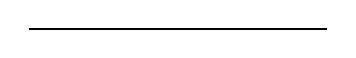
\begin{tikzpicture}
        \draw[thick] (0, 5cm) -- (3.79cm,5cm);
    \end{tikzpicture}
    
    % Chèn hình ảnh 
    \vspace{1em}
    \begin{figure}[H]
        \centering
        
\includegraphics[width=2.43cm, height=3.94cm]{image/Logo_Hust.png}
    \end{figure}
    
    % Tên Đồ án
    \vspace{1.5cm}
    {\sffamily \fontsize{21pt}{0pt}\selectfont {\textbf{ĐỒ ÁN TỐT NGHIỆP}}\\}
    \vspace{2em}
    {\sffamily \fontsize{17pt}{0pt}\selectfont {\textbf{THIẾT KẾ HỆ THỐNG TỰ ĐỘNG ĐIỀU CHỈNH NHIỆT ĐỘ TRONG THIẾT BỊ SẤY HOA QUẢ}}\\}
    % Tên 
    \vspace{2em}
    \textbf{\fontsize{11pt}{0pt}\selectfont LÊ ĐĂNG QUANG\\}
    \vspace{1ex}
    \fontsize{14pt}{0pt}\selectfont quang.ld224113@sis.hust.edu.vn\\

    \vspace{1em}
    \textbf{\fontsize{14pt}{0pt}\selectfont Ngành KT Điện tử \& Viễn thông\\}
    \vspace{1ex}
    \textbf{\fontsize{14pt}{0pt}\selectfont Chuyên ngành Điều khiển tự động \\}

    % Bảng thông tin
    \vspace{5em}
    \begin{tabular}{  l  l  r }
        \textbf{Giảng viên hướng dẫn:}&PGS. TS. Phạm Văn ABC& \fontsize{10pt}{0pt}\selectfont \stackon{Chữ ký của GVHD}{\rule{4cm}{0.4pt}} \\ [3em] 
        \textbf{Bộ môn:}&Điều khiển tự động& \\ [1ex] 
        \textbf{Trường:}&Điện - Điện tử& \\
    \end{tabular}

    % Thời gian
    \vfill

    \textbf{HÀ NỘI, 12/2019}
\end{center}
\cleardoublepage
 
    % NHIỆM VỤ ĐỒ ÁN TỐT NGHIỆP
% Bảng thông tin
\hspace*{-2cm} % Dịch chuyển bảng ra ngoài lề
\begin{tabular}{c c}
    BỘ GIÁO DỤC \& ĐÀO TẠO & \textbf{CỘNG HÒA XÃ HỘI CHỦ NGHĨA VIỆT NAM } \\ 
    \textbf{ĐẠI HỌC BÁCH KHOA HÀ NỘI} &\textbf{Độc lập - Tự do - Hạnh phúc }\\ 
\end{tabular}

\begin{center}
    \textbf{\centering NHIỆM VỤ\\}
    \textbf{\centering ĐỒ ÁN TỐT NGHIỆP\\}
\end{center}

{\centering Họ và tên sinh viên: \dotfill \\}
{\centering\makebox[\linewidth]{Khoa:\dotfill Viện:\dotfill Ngành:\dotfill}}
\textit{ % Bên trong in nghiêng
    \begin{enumerate}
        \item Tên đề tài:\\ .\dotfill
        \item Nội dung đề tài:\\ .\dotfill\\ .\dotfill\\ .\dotfill\\ .\dotfill\\ .\dotfill\\ .\dotfill\\ .\dotfill
        \item Cán bộ hướng dẫn:\\ \makebox[\linewidth]{Phần \hspace{7cm}  Họ tên cán bộ} \\  .\dotfill\\ .\dotfill\\ .\dotfill\\ .\dotfill
        \item Thời gian giao đề tài:\dotfill
        \item Thời gian hoàn thành đề tài:\dotfill
    \end{enumerate}
}
% Ngày tháng năm
\begin{flushleft}
    Ngày \makebox[1cm]{\dotfill} tháng \makebox[1cm]{\dotfill} năm \makebox{2024} \\
\end{flushleft}
\textbf{LÃNH ĐẠO BỘ MÔN}	 \hfill       \textbf{CÁN BỘ HƯỚNG DẪN}\\ 

\vspace{1.5cm}
\begin{center}
    \textbf{SINH VIÊN THỰC HIỆN\\}
    \textit{{(Ký và ghi rõ họ tên)}}
\end{center}
\thispagestyle{empty}
\cleardoublepage 
    \thispagestyle{empty}

\subsection*{\centering Lời cảm ơn}
Đây là mục tùy chọn, nên viết phần cảm ơn ngắn gọn, tránh dùng các từ sáo rỗng, giới hạn trong khoảng 100-150 từ. 

\subsection*{\centering Tóm tắt nội dung đồ án}
Tóm tắt nội dung của đồ án tốt nghiệp trong khoảng tối đa 300 chữ. Phần tóm tắt cần nêu được các ý: vấn đề cần thực hiện; phương pháp thực hiện; công cụ sử dụng (phần mềm, phần cứng…); kết quả của đồ án có phù hợp với các vấn đề đã đặt ra hay không; tính thực tế của đồ án, định hướng phát triển mở rộng của đồ án (nếu có); các kiến thức và kỹ năng mà sinh viên đã đạt được.


\vfill
\begin{tabularx}{\textwidth}{>{\centering\arraybackslash}X>{\centering\arraybackslash}X}
    \centering
    & Sinh viên thực hiện \\
    \centering
    &\fontsize{10pt}{0}\selectfont Ký và ghi rõ họ tên \\
    \centering
\end{tabularx}
  
\cleardoublepage 
    % MỤC LỤC
\addtocontents{toc}{\protect\thispagestyle{empty}}
\tableofcontents % tạo mục lục tự dộng 
\thispagestyle{empty}
\cleardoublepage

% DANH MỤC KÝ HIỆU VÀ CHỮ VIẾT TẮT
\pagenumbering{roman} % Đánh số thứ tự la mã
\section*{\centering DANH MỤC KÝ HIỆU VÀ CHỮ VIẾT TẮT}
\phantomsection \addcontentsline{toc}{section}{\numberline {} DANH MỤC KÝ HIỆU VÀ CHỮ VIẾT TẮT}
\begin{tabular}{ l l }
\hspace{1cm} AWGN & \hspace{4cm} Additive White Gaussian Noise \\  
\hspace{1cm} BC & \hspace{4cm} Broadcast Channel    \\
\hspace{1cm} BS  & \hspace{4cm} Base Station\\
\hspace{1cm} CSI & \hspace{4cm} Channel State Information \\  
\end{tabular}  
\cleardoublepage

% DANH MỤC HÌNH VẼ
{
    \let\oldnumberline\numberline%
    \renewcommand{\numberline}{\figurename~\oldnumberline}%
    \listoffigures%
}
\phantomsection\addcontentsline{toc}{section}{\numberline {} DANH MỤC HÌNH VẼ}
\cleardoublepage

% DANH MỤC BẢNG BIỂU
{
    \let\oldnumberline\numberline%
    \renewcommand{\numberline}{\tablename~\oldnumberline}%
    \listoftables%
}
\phantomsection\addcontentsline{toc}{section}{\numberline {} DANH MỤC BẢNG BIỂU}
\cleardoublepage 
    \pagenumbering{arabic}
\phantomsection\section*{\centering CHƯƠNG 1.	CÁC QUI ĐỊNH CHUNG}
\addcontentsline{toc}{section}{\numberline{}CHƯƠNG 1. CÁC QUI ĐỊNH CHUNG}
\setcounter{section}{1}
\setcounter{subsection}{0}
\setcounter{figure}{0}
\setcounter{table}{0}
Phần mở đầu giới thiệu vấn đề mà đồ án cần giải quyết mô tả được các phương pháp hiện có để giải quyết vấn đề, trình bày mục đích của đồ án song song với việc giới hạn phạm vi của vấn đề mà đồ án tập chung giải quyết. Phần này cũng giới thiệu tóm tắt cấu trúc đồ án và nội dung tương ứng của các phần sẽ lần lượt được trình bày ở các chương tiếp theo.

Nội dung chính của 1 đồ án tốt nghiệp bao gồm:
\begin{itemize}
    \item Phần mở đầu giới thiệu đề tài.
    \item Một chương giới thiệu cơ sở lý thuyết.
    \item Một hoặc nhiều chương trình bày các vấn đề về tính toán và thiết kế.
    \item Một chương mô tả các thí nghiệm và kết quả thu được.
\end{itemize}


\cleardoublepage
\phantomsection\section*{\centering CHƯƠNG 2. SỬ DỤNG CÁC BIỂU ĐỒ}
\addcontentsline{toc}{section}{\numberline{}CHƯƠNG 2. SỬ DỤNG CÁC BIỂU ĐỒ}
\setcounter{section}{2}
\setcounter{subsection}{0}
\setcounter{figure}{0}
\setcounter{table}{0}
Mỗi chương sẽ bắt đầu bằng đoạn giới thiệu các phần chính được trình bày trong chương đó, dài khoảng 5 - 10 dòng và kết thúc bằng 1 đoạn tóm tắt các kết luận chính của chương. Chú ý phân bổ chiều dài của mỗi chương cho cân đối và hợp lý 
\subsection{Một số lưu ý khi trình bày đồ án}
Sau đây là 1 vài chú ý khi làm đồ án các bạn cần nhớ nhé
\subsubsection{Nộp đồ án}
Sinh viên (hoặc nhóm sinh viên tối đa 3 thành viên làm chung 1 đề tài) phải nộp 2 quyển đồ án tốt nghiệp tại văn phòng bộ môn của giảng viên hướng dẫn trước ngày bảo vệ ít nhất 1 tuần. Một quyển đồ án cần có các đặc điểm sau:
\begin{itemize}
    \item Được \textbf{in 2 mặt} nhằm tiết kiệm không gian lưu trữ.
    \item Đóng bìa mềm, bên ngoài là bóng kính. 
    \item Số trang 50 - 150 trang, không kể phần phục lục
    \item Phải có chữ ký của sinh viên sau lời cam đoan và của giảng viên hướng dẫn. 
\end{itemize}
\subsubsection{Phụ lục}
Phụ lục nếu có chứa thông tin có liên quan đến đồ án nhưng nếu để trong phần chính sẽ gây rườm rà. Thông thường các chi tiết để trong phần phụ lục là kết quả thô (chưa qua xử lý), mã nguồn phần mềm, thông số chi tiết của linh kiện hoặc hình thành minh họa thêm...
\subsubsection{Tài liệu tham khảo}
\paragraph{Cách liệt kê} \mbox{} % mbox để xuống dòng 

Áp dụng cách liệt kê theo quy định của IEEE. Theo đó tài liệu tham khảo được đánh số thứ tự trong ngoặc vuông. Thứ tự liệt kê là thứ tự xuất hiện của tài liệu tham khảo được trích dẫn trong đồ án. Tài liệu tham khảo đã liệt kê bắt buộc phải được trích dẫn trong phần nội dung của đồ án. Tài liệu tham khảo cần có nguồn gốc rõ ràng và phải từ nguồn đáng tin cậy. Cần hạn chế trích dẫn tài liệu tham khảo từ các website, từ wikipedia.
\paragraph{Các loại tài liệu tham khảo} \mbox{} % mbox để xuống dòng 

Các nguồn tài liệu tham khảo chính là sách, bài báo trong các tạp chí, bài báo trong các hội nghị khoa học và các tài liệu tham khảo khác trên internet.
\subsubsection{Đánh số phương trình}
Phương trình được đánh số theo số của chương, như hình vẽ và bảng biểu.
\subsubsection{Đánh số định nghĩa, định lý, hệ quả}
Các định nghĩa định lý hệ quả sẽ được đánh số theo số của chương và được sử dụng chung 1 chỉ số. Ví dụ trong chương 3, các định nghĩa, định lý, hệ quả sẽ được đánh số theo thứ tự: Định lý 3.1 , Định nghĩa 3.2, Hệ quả 3.3, Định lý 3.4...

\cleardoublepage
\phantomsection\section*{\centering CHƯƠNG 3. THUẬT TOÁN}
\addcontentsline{toc}{section}{\numberline{}CHƯƠNG 3. THUẬT TOÁN}
\setcounter{section}{3}
\setcounter{subsection}{0}
\setcounter{figure}{0}
\setcounter{table}{0}
Đây \cite{stein2011fourier} là phần sinh viên tự phát triển như xây dựng thuật toán, xây dựng chương trình, mô phỏng, tính toán, thiết kế, chạy thử kết quả... \cite{howell2016principles}
\subsection{Cách chèn ảnh}
\begin{figure}[H]
    \centering
    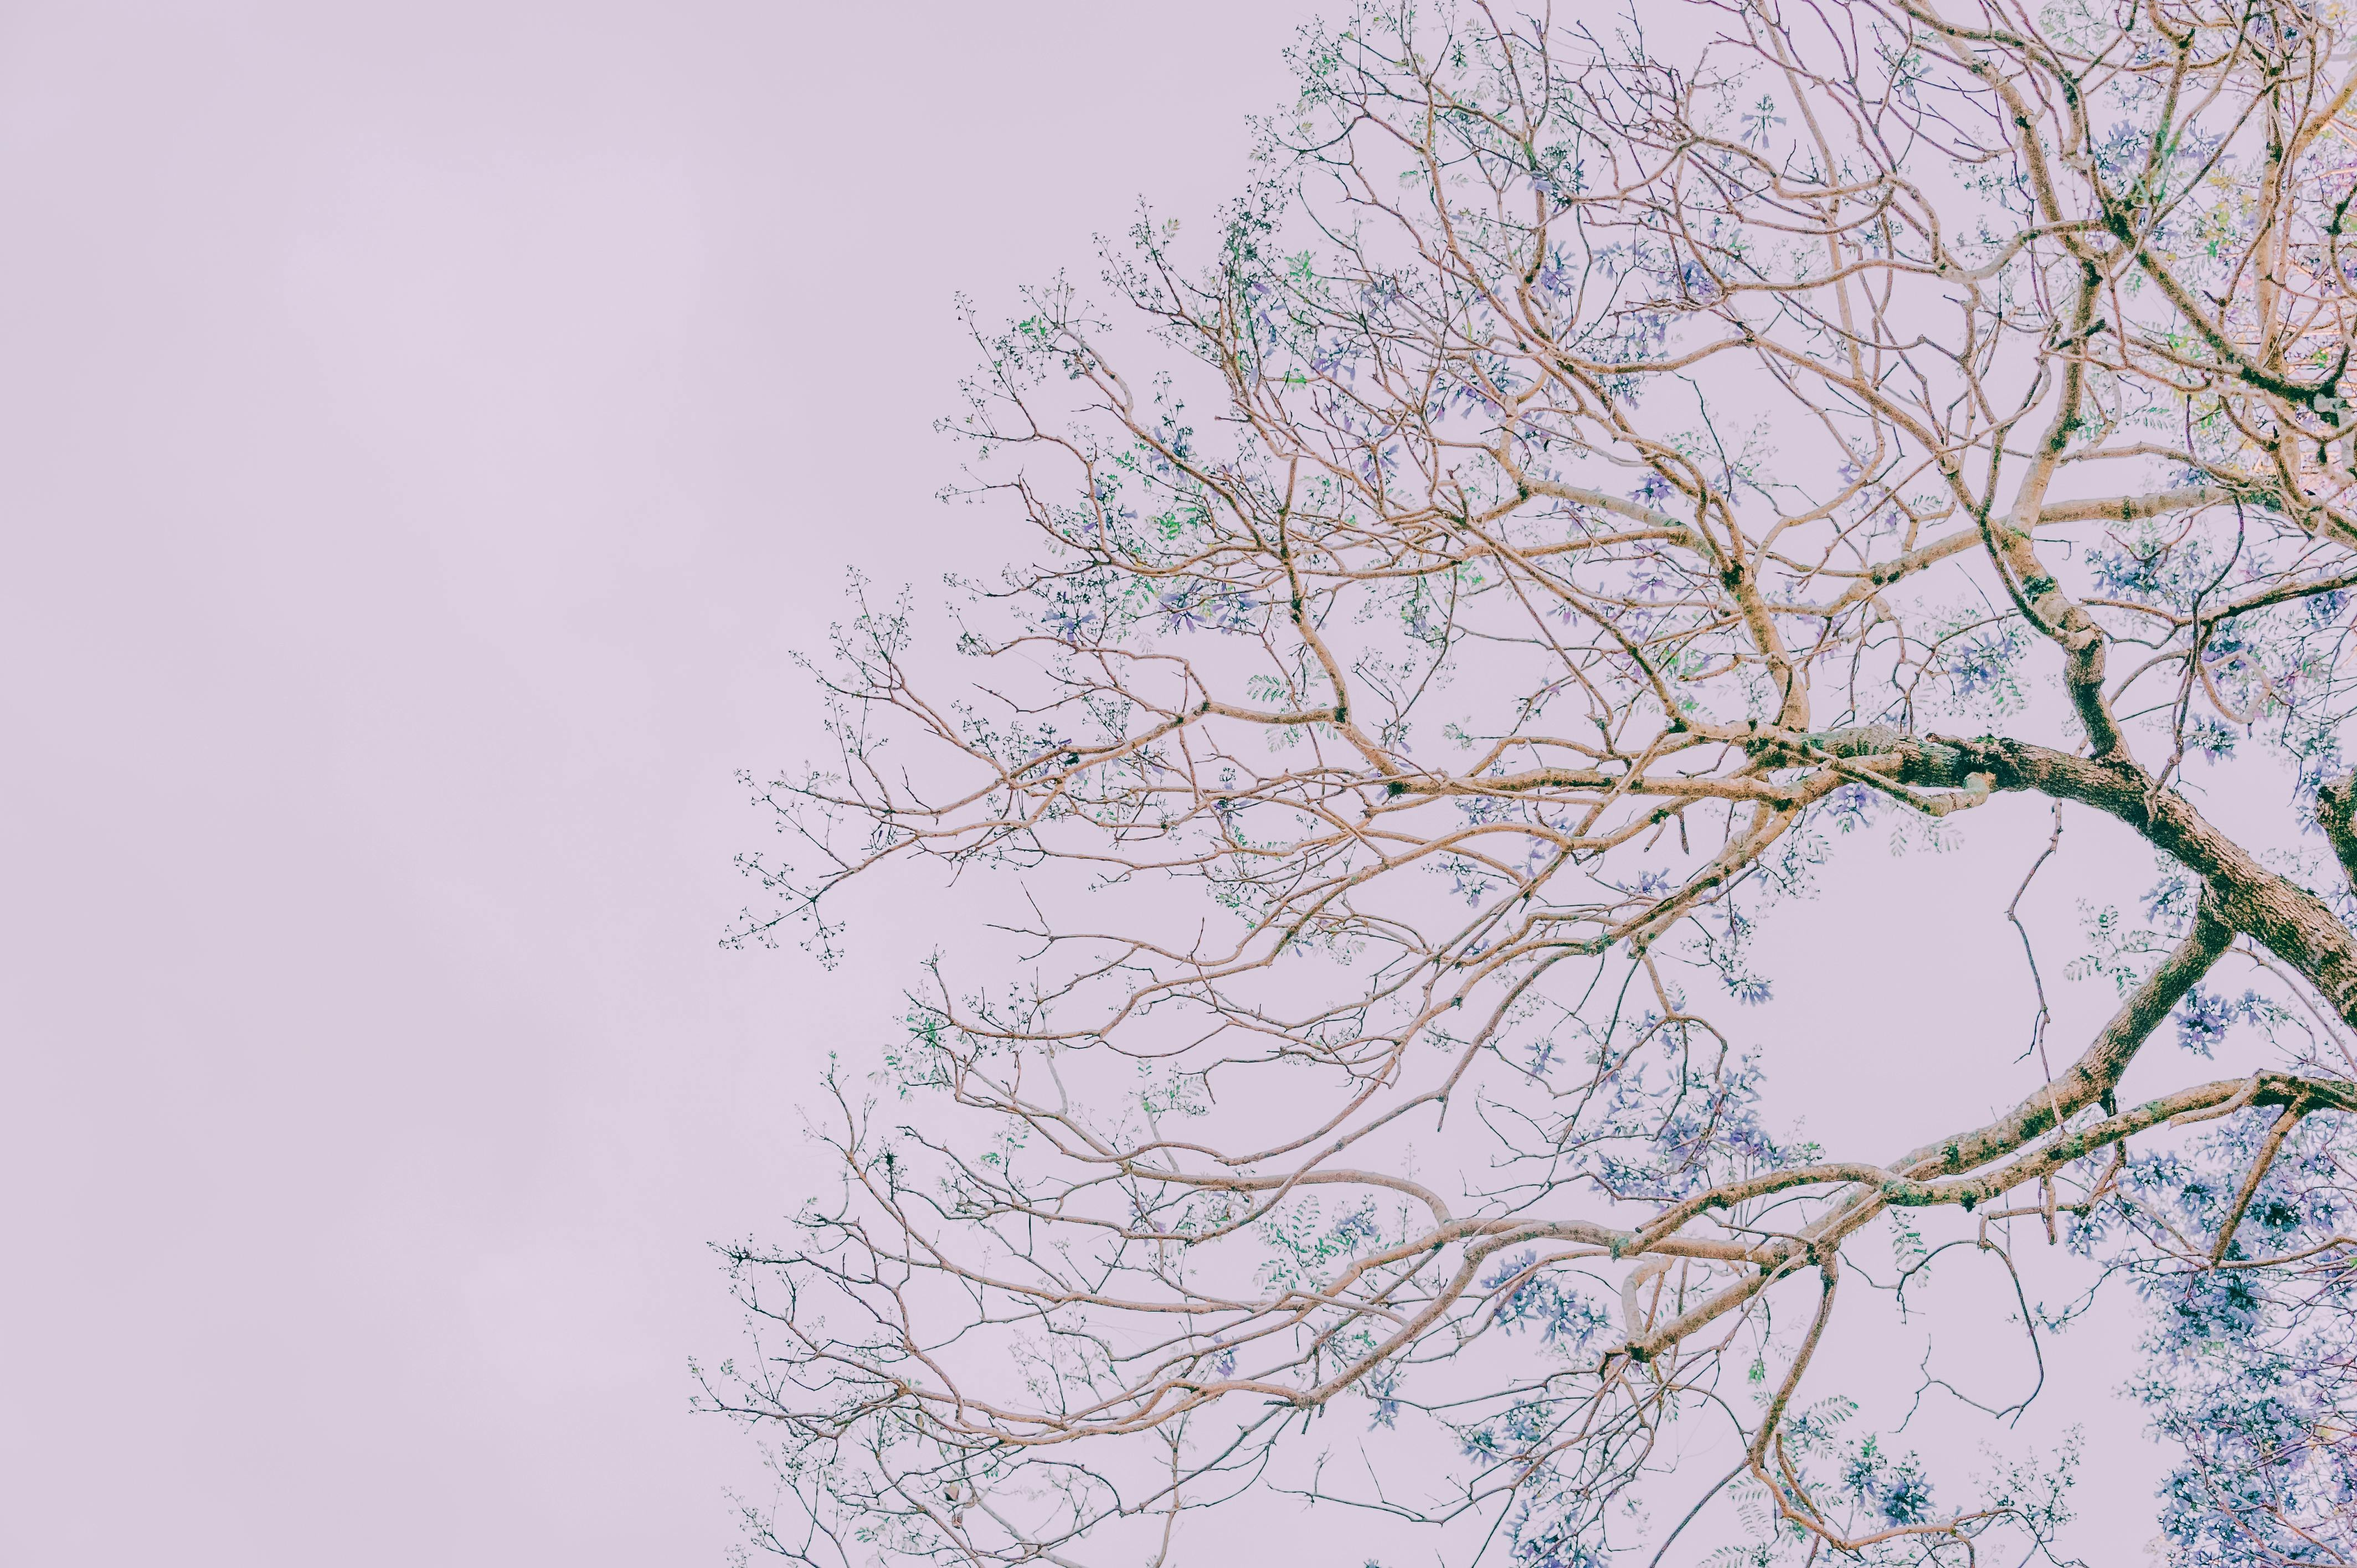
\includegraphics[width=0.75\textwidth, height=4.39cm]{image/Tree.jpg}
    \caption[Sơ đồ khối của hệ thống]{\textit{\fontsize{12pt}{0}\selectfont Sơ đồ khối của hệ thống}}
    \label{hinh31}
\end{figure}
Hình \ref{hinh31} là ví dụ về cách chèn ảnh. Lưu ý chú thích của hình vẽ được đặt ngay dưới hình vẽ. Tất cả các hình vẽ phải được đề cập đến trong phần nội dung và phải được phân tích và bình luận giống mình đang làm thế này nhé hihi :)

\subsection{Cách tạo bảng}
\begin{table}[H]
    \centering
    \caption[Kết quả thí nghiệm]{\textit{\fontsize{12pt}{0}\selectfont Kết quả thí nghiệm}}
    \begin{tabularx}{0.75\textwidth}{
        |>{\centering\arraybackslash}s
        |>{\centering\arraybackslash}a
        |>{\centering\arraybackslash}a
        |>{\centering\arraybackslash}s|
        }
        \hline
        \bfseries Lần thí nghiệm & \bfseries Điện áp đo được (mV) &\bfseries Điện áp tham chiếu (mV)& \bfseries Sai lệch (\%)\\\hline
        1&&&\\\hline
        2&&&\\\hline
        3&&&\\\hline
    \end{tabularx}
    \label{bang31}
\end{table}
Bảng \ref{bang31} là ví dụ về cách tạo bảng. Lưu ý chú thích của bảng được đặt ở trước bảng. Tất cả các bảng biểu phải được đề cập đến trong phần nội dung và phải phân tích và bình luận giống như mình đang làm nhé hehe :)

\subsection{Cách viết phương trình}
\begin{equation}
    \label{pt31}
    F(x) = \int^a_b \frac{1}{3}x^3
\end{equation}
Phương trình \ref{pt31} là ví dụ về phương trình tích phân.

Thử phương trình khác 
\begin{equation}
    \label{pt32}
    x[t_n] = \frac{1}{\sqrt{n}} \sum_{k=0}^{N-1}[f_k]
\end{equation}
Phương trình \ref{pt32} là phương trình biến đổi Fourier
\subsection{Cách viết định nghĩa, định lý, hệ quả, bổ đề...}
Định lý lấy mẫu Nq-shannon là một định lý được sử dụng trong lĩnh vực lý thuyết thông tin đặc biệt là trong viễn thông và xử lý tín hiệu 
\begin{theorem} % Định lý
    \label{dlNq}
    Một hàm số tín hiệu  $x(t_n)$ không chứa bất kỳ thành phần tần số nào lớn hơn hoặc bằng 1 giá trị $f_m$ có thể biểu diễn chính xác bằng tập các giá trị của nó với chu kỳ lấy mẫu $T = 1/(2f_m)$.
\end{theorem}
Định lý \ref{dlNq} thường được gọi đơn giản là định lý lấy mẫu 
\begin{corollary}
    Một người có thể làm được thì sẽ nghĩ mình làm đư
\end{corollary}
\begin{lemma}
    Một người có thể làm được thì sẽ nghĩ mình làm đư
\end{lemma}
\begin{defn}
    \label{defn}
    Một người có thể làm được thì sẽ nghĩ mình làm đư
\end{defn}
Định nghĩa \ref{defn} được nhắc tới như là tiếng gọi hoang rã từ nơi không người
\cleardoublepage

\phantomsection\section*{\centering CHƯƠNG 4. THÍ NGHIỆM VÀ KẾT QUẢ}
\addcontentsline{toc}{section}{\numberline{} CHƯƠNG 4. THÍ NGHIỆM VÀ KẾT QUẢ}
\setcounter{section}{4}
\setcounter{subsection}{0}
\setcounter{figure}{0}
\setcounter{table}{0}
\subsection{Sao nó không đúng?}
\lipsum
\begin{figure}[H]
    \centering
    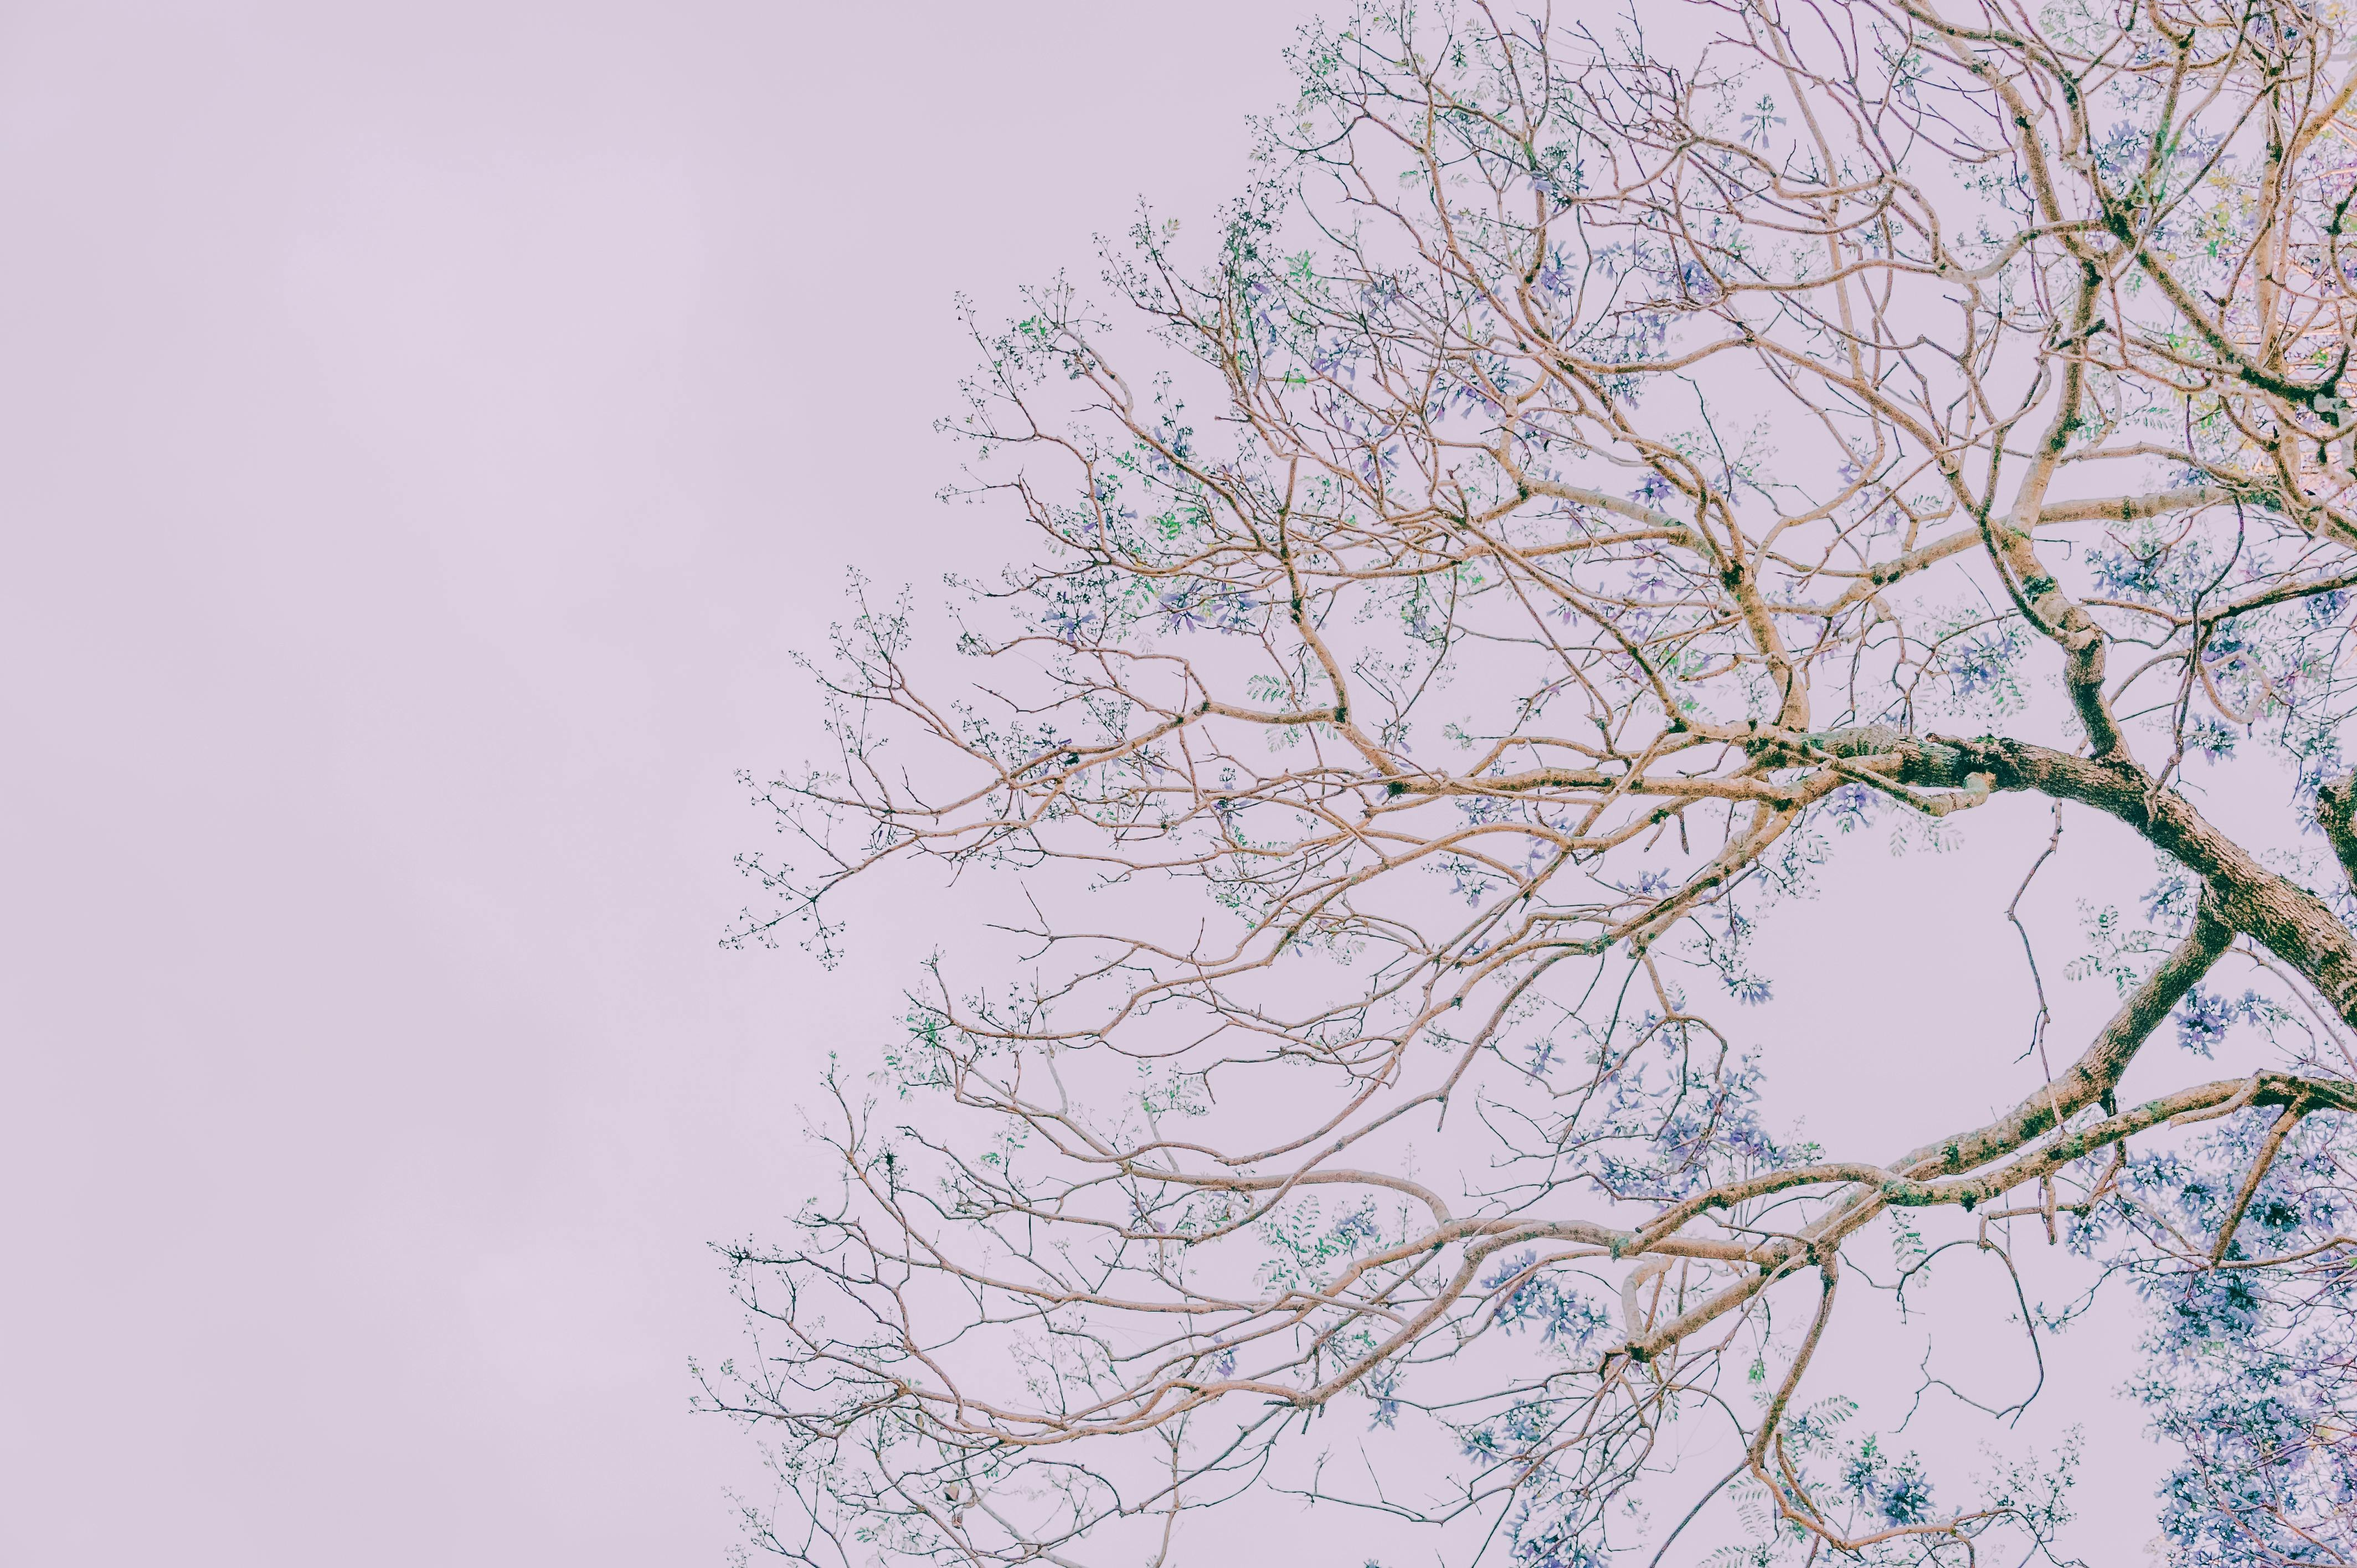
\includegraphics[width=0.75\textwidth, height=4.39cm]{image/Tree.jpg}
    \caption[Sơ đồ khối của hệ thống]{\textit{\fontsize{12pt}{0}\selectfont Sơ đồ khối của hệ thống}}
    \label{hinh4.1}
\end{figure}
Hình \ref{hinh4.1} đây là ví dụ về cách chèn ảnh. Và cách chèn tài liệu tham khảo \cite{bracewell1989fourier}
\cleardoublepage 
    \phantomsection\section*{\centering KẾT LUẬN}
\addcontentsline{toc}{section}{\numberline{}KẾT LUẬN}

\phantomsection\subsection*{Kết luận chung}
\addcontentsline{toc}{section}{\numberline{}Kết luận chung}
Kết luận chung cho các chương trong đồ án. Mục này cần nhấn mạnh những vấn đề cần giải quyết và vấn đề chưa giải quyết để đưa ra đánh giá về mức độ hoàn thành công việc đánh giá này bao gồm so sánh kết quả thu được với mục tiêu đề ra ban đầu.

\phantomsection\subsection*{Hướng phát triển}
\addcontentsline{toc}{section}{\numberline{}Hướng phát triển}

\phantomsection\subsection*{Kiến nghị và đề xuất (nếu có)}
\addcontentsline{toc}{section}{\numberline{}Kiến nghị và đề xuất (nếu có)}

\cleardoublepage 
    \phantomsection\addcontentsline{toc}{section}{\numberline{}TÀI LIỆU THAM KHẢO}
\bibliographystyle{IEEEtran}
\bibliography{KetThuc/TaiLieuThamKhao}
\cleardoublepage 
    \phantomsection\section*{\centering PHỤ LỤC}
\addcontentsline{toc}{section}{\numberline{}PHỤ LỤC}


\texttt{\fontsize{10pt}{0pt}\selectfont Mã nguồn chương trình (nếu có) dược đưa vào đây sử dụng font Courier New, cỡ 10pt}

\begin{enumerate}[label=\textbf{A\arabic*.}]
  
    \item  \textbf{Chi tiết số liệu thí nghiệm}
    
    Trình phụ lục tại đây (nếu có). Trình phụ lục tại đây (nếu có). Trình phụ lục tại đây (nếu có). Trình phụ lục tại đây (nếu có). Trình phụ lục tại đây (nếu có). Trình phụ lục tại đây (nếu có). Trình phụ lục tại đây (nếu có). Trình phụ lục tại đây (nếu có). Trình phụ lục tại đây (nếu có). Trình phụ lục tại đây (nếu có). Trình phụ lục tại đây (nếu có). Trình phụ lục tại đây (nếu có).
    \item  \textbf{Chi tiết các bước tính toán}
    
    Trình phụ lục tại đây (nếu có). Trình phụ lục tại đây (nếu có). Trình phụ lục tại đây (nếu có). Trình phụ lục tại đây (nếu có). Trình phụ lục tại đây (nếu có). Trình phụ lục tại đây (nếu có). Trình phụ lục tại đây (nếu có). Trình phụ lục tại đây (nếu có). Trình phụ lục tại đây (nếu có). Trình phụ lục tại đây (nếu có). Trình phụ lục tại đây (nếu có). Trình phụ lục tại đây (nếu có).
    \item  \textbf{Chi tiết sơ đồ mô phỏng}
    
    Trình phụ lục tại đây (nếu có). Trình phụ lục tại đây (nếu có). Trình phụ lục tại đây (nếu có). Trình phụ lục tại đây (nếu có). Trình phụ lục tại đây (nếu có). Trình phụ lục tại đây (nếu có). Trình phụ lục tại đây (nếu có). Trình phụ lục tại đây (nếu có). Trình phụ lục tại đây (nếu có). Trình phụ lục tại đây (nếu có). Trình phụ lục tại đây (nếu có). Trình phụ lục tại đây (nếu có).
    
\end{enumerate} 
\end{document}